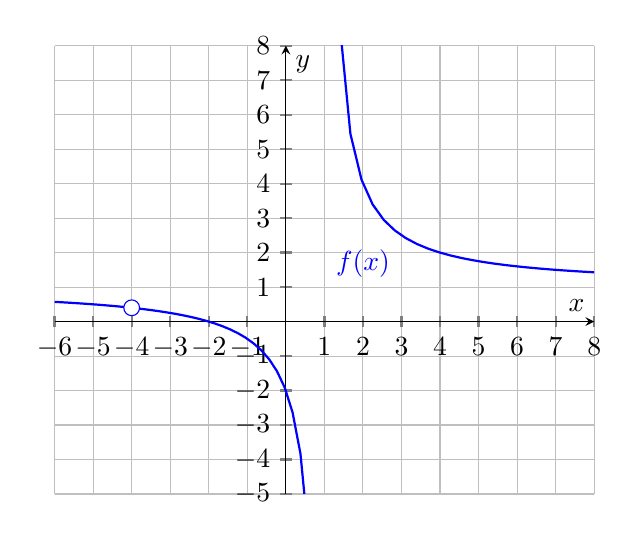
\begin{tikzpicture}[scale=1]
    \begin{axis}[
        axis lines=middle,
        grid=major,
        xmin=-6, xmax=8,
        ymin=-5, ymax=8,
        xtick={-6,-5,...,8},
        ytick={-5,-4,...,8},
          tick style={thick},
        ylabel=$y$,
        xlabel=$x$,
            ]
        \addplot[domain=-6:-4.1, blue,  thick] {(x^2+6*x+8)/(x^2+3*x-4)};
         \addplot[domain=-3.9:0.99, blue,  thick] {(x^2+6*x+8)/(x^2+3*x-4)};
           \addplot[domain=1.1:8, blue,  thick] {(x^2+6*x+8)/(x^2+3*x-4)};
        \addplot[mark=none, color=blue, nodes near coords={$f(x)$}] coordinates {(2,1)};
          \draw[fill=white, draw=blue](axis cs:-4,0.4) circle(1mm);
    \end{axis}
    \end{tikzpicture}